\documentclass{beamer}
\usepackage{beamerthemeshadow}
\usepackage[utf8]{inputenc} % set input encoding (not needed with XeLaTeX)
\usepackage[T1]{fontenc}
\usepackage[francais]{babel}
\usepackage{listings}


% ---- PAGE NUMBER ----
\setbeamertemplate{footline}%{miniframes theme}
{%
	\begin{beamercolorbox}[colsep=1.5pt]{upper separation line foot}
	\end{beamercolorbox}
	\begin{beamercolorbox}[ht=2.5ex,dp=1.125ex,%
		leftskip=.3cm,rightskip=.3cm plus1fil]{author in head/foot}%
		\leavevmode{\usebeamerfont{author in head/foot}\insertshortauthor}%
		\hfill%
		{\usebeamerfont{institute in head/foot}\usebeamercolor[fg]{institute in head/foot}\insertshortinstitute}%
		{\usebeamerfont{title in head/foot}\insertshorttitle} \hfill     \insertframenumber%
	\end{beamercolorbox}%
	\begin{beamercolorbox}[colsep=1.5pt]{lower separation line foot}
	\end{beamercolorbox}
}

%$HeadURL: https://subversion.assembla.com/svn/cfpt-courses/trunk/_inc/inc_lst_csharp.tex $
%$LastChangedDate: 2014-01-22 11:03:53 +0100 (mer., 22 janv. 2014) $
%$LastChangedRevision: 5197 $
%$LastChangedBy: marechal $

% lstlisting configuration for C#
%-------------------------------------------------------------------------------------
\usepackage{xcolor}
\usepackage{listings}
\usepackage{accsupp}

% color
\definecolor{lightgreen}{rgb}	{0.200, 0.980, 0.200}
\definecolor{darkgreen}{rgb}	{0.000, 0.400, 0.000}
\definecolor{lightgray}{gray}	{0.98}
\definecolor{darkred}{rgb}		{0.545, 0.000, 0.000}

% CSharp colors
\definecolor{class}{rgb}		{0.200, 0.600, 0.600}	% Cyan Visual Studio
\definecolor{keyword}{rgb}		{0.000, 0.000, 1.000}	% blue

% code to avoid line number copy during copy-paste from PDF
\newcommand{\noncopynumber}[1]{%
    \BeginAccSupp{method=escape,ActualText={}}%
    {\scriptsize#1}%
    \EndAccSupp{}%
}

% lstlisting parameters
\lstset {	
  language=[Sharp]C
, captionpos=b
, frame=shadowbox
, rulesepcolor=\color{gray}
% syntaxic coloration
, basicstyle=\footnotesize\ttfamily
, keywordstyle=\color{blue}
, commentstyle=\color{darkgreen}
, stringstyle=\color{darkred}
, backgroundcolor=\color{lightgray}
, identifierstyle=\color{black}
% lines numbering
, numbers=left
, numberstyle=\noncopynumber
, stepnumber=1
, numbersep=5pt
%
, breaklines=true
, tabsize=2
, showstringspaces=false
, lineskip={-1.5pt} % single line spacing
, escapeinside={/*(*@}{@*)*/}
, rangeprefix=\{\  % curly left brace plus space
, rangesuffix=\ \} % space plus curly right brace
}

% Csharp : additional keywords
\lstset{
	morekeywords={var,get,set,string,value},
	otherkeywords={\#region,\#endregion,\#define,\#if,\#endif,\#else}, %morekeyword does not support # chararacter then we must use otherkeywords
	emph={[1]Application,
		Char,Color,Console,Convert,
		DialogResult,
		Environment,EventArgs,
		Form,
		Object,String,
		SByte,Int16,Int32,Int64,
		Byte,UInt16,UInt32,UInt64,
		Single,Double,
		Keys,KeyPressEventArgs,
		MessageBox,MessageBoxButtons},
	emphstyle={[1]\color{class}}
}

\lstset{prebreak=\raisebox{0ex}[0ex][0ex]
        {\ensuremath{\hookleftarrow}}}
%\lstset{postbreak=\raisebox{0ex}[0ex][0ex]
%        {\ensuremath{\hookrightarrow\space}}}
\lstset{breaklines=true, breakatwhitespace=true}

% replace sequence of char by another sequence of char
% see http://stackoverflow.com/questions/1116266/listings-in-latex-with-utf-8-or-at-least-german-umlauts
\lstset{literate=%
{ä}{{\"a}}1
{â}{{\^a}}1
{à}{{\`a}}1
{Ä}{{\"A}}1
{Â}{{\^A}}1
{À}{{\`A}}1
{ë}{{\"e}}1
{ê}{{\^e}}1
{é}{{\'e}}1
{è}{{\`e}}1
{Ë}{{\"E}}1
{Ê}{{\^E}}1
{É}{{\'E}}1
{È}{{\`E}}1
{ï}{{\"i}}1
{î}{{\^i}}1
{Ï}{{\"I}}1
{Î}{{\^I}}1
{ö}{{\"o}}1
{ô}{{\^o}}1
{Ö}{{\"O}}1
{Ô}{{\^O}}1
{ü}{{\"u}}1
{û}{{\^u}}1
{ù}{{\`u}}1
{Ü}{{\"U}}1
{Û}{{\^U}}1
{Ù}{{\`U}}1
{ç}{{\c c}}1
{Ç}{{\c C}}1
{°}{{\textsuperscript{o}}}1
% suppress BOM (Byte Order Mark) characters at the beginning of Visual Studio source
% see http://tex.stackexchange.com/questions/5935/how-to-suppress-bom-effect-in-the-output
{�}{}0
{�}{}0
{�}{}0
}


\begin{document}
\title{Web Media Manager}  
\author{Jean-Philippe Froelicher}
\date{\today} 

\frame{\titlepage \centering Centre de Formation Professionnel Technique} 

\frame{\frametitle{Sommaire}\tableofcontents[hideallsubsections]} 

\section{Introduction} 
\subsection{Média vidéo du Web}
\frame{\frametitle{Média vidéo du Web} 
	\begin{itemize}
		\item Plate-forme d'hébergement vidéo.
		\item Twitch ; Youtube ; Dailymotion ; Vimeo ; Ustream etc.
		\item Vidéo à la demande (VOD) ; diffusion de flux vidéo en direct.
		\item Rémunération suivant le nombres de vues ; dons.
	\end{itemize}
	\begin{columns}
		\column{0.3\textwidth}
		\begin{figure}[h]
			\center
			
\includegraphics[width=0.8\textwidth]{youtube.png}
		\end{figure}
		\column{0.3\textwidth}
		\begin{figure}[h]
			\center
			
\includegraphics[width=0.8\textwidth]{twitch.png}
		\end{figure}
		\column{0.3\textwidth}
		\begin{figure}[h]
			\center
			
\includegraphics[width=0.8\textwidth]{dailymotion.png}
		\end{figure}
	\end{columns}
}

\subsection{Sujet}
\frame{\frametitle{Sujet} 
\begin{itemize}
	\item Projet de diplôme
	\item Agrégateur de sites
		\begin{itemize}
			\item Reproduis les mêmes fonctions
			\item Ajout de fonctions
			\item Évolutive et souple
		\end{itemize}
	\item Langage C\#
\end{itemize}
}

\section{Principales fonctionnalités} 
\subsection{Fonctions de bases}
\frame{\frametitle{Fonctions de bases} 
	Chaque site intègre ces fonctions :
	\begin{itemize}
		\item Connexion à un compte
		\item Visionnage d'une vidéo / vidéo en direct
		\item S'abonner à une chaîne
		\item Chat IRC pour les vidéos en direct
		\item Recherche de vidéos
		\item Vidéos actuellement en direct ; dernières vidéos
		\item Chaînes abonnées
	\end{itemize}
}
\subsection{Notifications}
\frame{\frametitle{Notifications} 
	Une notification apparaît lorsqu'une vidéo sort ou qu'une nouvelle diffusion en direct commence
	\begin{itemize}
		\item Pop-up qui apparaît avec les informations de la vidéo.
	\end{itemize}
	Les notifications sont activées uniquement pour les chaînes que l'utilisateur suit.
	\begin{figure}[h]
		\center
		
\includegraphics[width=0.7\textwidth]{notificationview.png}
	\end{figure}
}
\subsection{Chat IRC}
\frame{\frametitle{Chat IRC} 
	\begin{columns}
		\column{0.5\textwidth}
		Internet Relay Chat, Protocole de communication textuelle.
		Uniquement sur les vidéos en direct.

		\column{0.5\textwidth}
		\begin{figure}[h]
			\center
			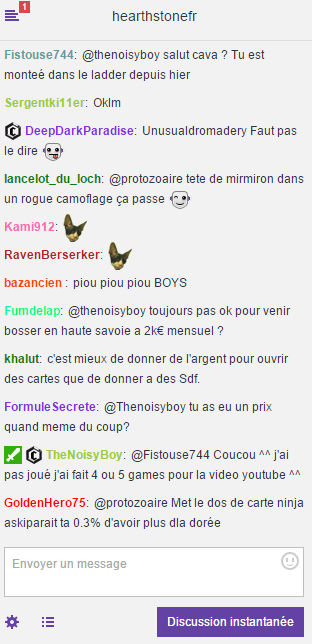
\includegraphics[width=0.8\textwidth]{chatIrc.png}
		\end{figure}
	\end{columns}	
}
\subsection{Catégorie \& Liste de lecture}
\frame{\frametitle{Catégorie \& Liste de lecture} 
	Une catégorie sert à rassembler des vidéos de différents sites au même endroit.\\
	Une liste de lecture lit les vidéos qu'elle contient à la suite.

}


\section{Mise en oeuvre}
\subsection{Conception}
\frame{\frametitle{Conception} 
	\begin{figure}[h]
		\center
		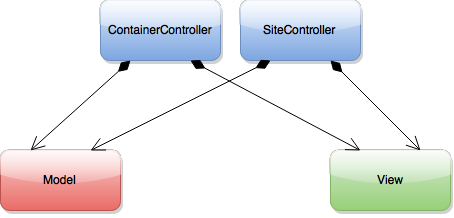
\includegraphics[width=0.8\textwidth]{mvc.png}
	\end{figure}
}
\frame{\frametitle{Conception} 
	\begin{figure}[h]
		\center
		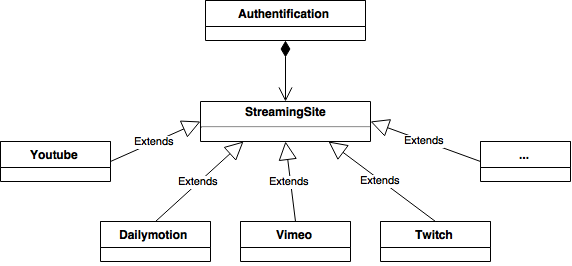
\includegraphics[width=1\textwidth]{StreamingSite.png}
	\end{figure}
}
\subsection{SVideo \& SChannel}
\begin{frame}
	\frametitle{SVideo \& SChannel}
	\begin{columns}
		\column{0.5\textwidth}
		\begin{itemize}
			\item Structure
				\begin{itemize}
					\item Informations communes
				\end{itemize}
			\item Vidéo et chaîne
			\item Type générique
		\end{itemize}
		
		\column{0.5\textwidth}
		\begin{figure}[h]
			\center
			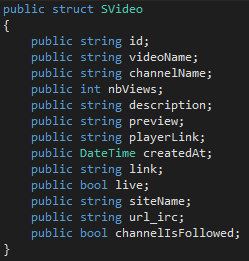
\includegraphics[width=0.9\textwidth]{SVideo.png}
		\end{figure}
	\end{columns}	
\end{frame}

\subsection{Récupération des données}
\frame{\frametitle{Récupération des données} 
	\begin{figure}[h]
		\center
		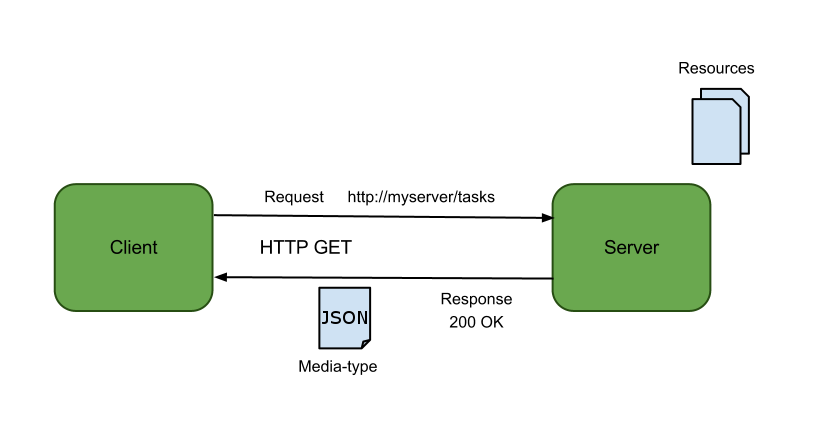
\includegraphics[width=1\textwidth]{rest.png}
	\end{figure}	
}

\frame{\frametitle{Json} 
	\begin{figure}[h]
		\center
		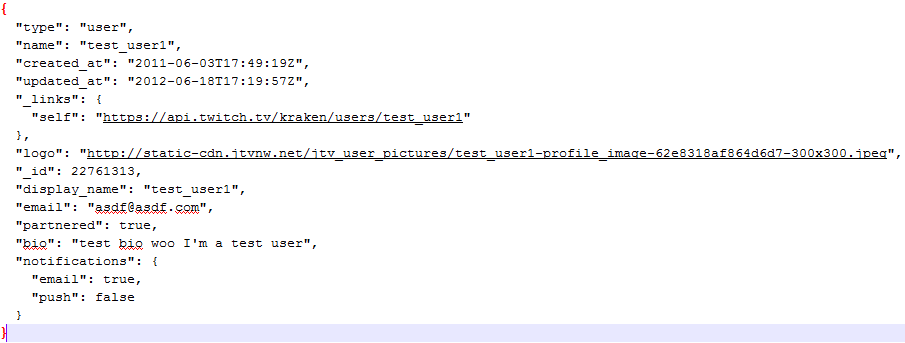
\includegraphics[width=1\textwidth]{json.png}
	\end{figure}	
	Exemple de données formaté en Json.
}

\frame{\frametitle{Classes structures}
	\begin{columns}
		\column{0.5\textwidth}
		Afin de recevoir les données dans un bon type, il faut créer des classes structures pour chaque site.
		
		\column{0.5\textwidth}
		\begin{figure}[h]
			\center
			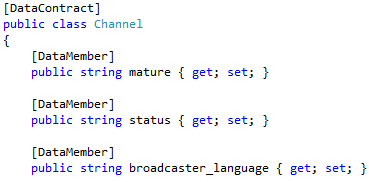
\includegraphics[width=1\textwidth]{ChannelTwitch.png}
		\end{figure}
	\end{columns}
}

\frame{\frametitle{Désérialisation} 
	Un objet est créé depuis les données formaté en Json.\\
	Type générique et lors de l'appel de la méthode, on indique une classe structure.
	\begin{figure}[h]
		\center
		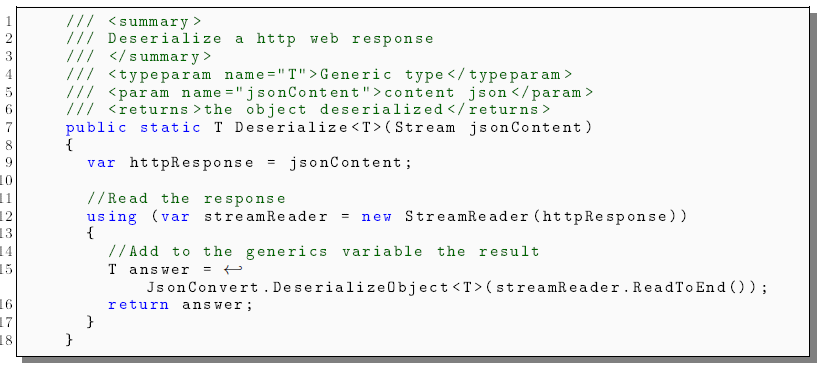
\includegraphics[width=0.9\textwidth]{deserialize.png}
	\end{figure}
}

\frame{\frametitle{Cycle d'un accès} 
	\begin{figure}[h]
		\center
		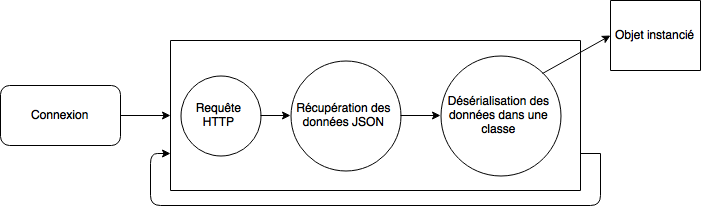
\includegraphics[width=0.9\textwidth]{cycle.png}
	\end{figure}
}

\subsection{Connexion}
\frame{\frametitle{Connexion} 
	\begin{itemize}
		\item Avoir un compte existant sur le site
		\item Connexion grâce au protocole OAuth2
		\item Utilisation du lien de connexion de l'API
		\begin{itemize}
			\item \textcolor{blue}{api.twitch.tv/kraken/oauth2/authorize}?\textcolor{red}{response\_type=token}
			\&\textcolor{darkgreen}{client\_id= 9jfbie2pedk3xzoj3s53268v7fb4zds}
			\&\textcolor{orange}{redirect\_uri= https://froelicher.github.io/WebMediaManager/WebSite}
			\&\textcolor{violet}{scope=user\_read+channel\_read}
		\end{itemize}
		\item Récupération du jeton d'accès dans l'url de redirection
		\begin{itemize}
			\item Création d'un GitHub Page
		\end{itemize}
	\end{itemize}
	
}

\subsection{Notifications}
\frame{\frametitle{Notifications} 
	Vérification toutes les 5 secondes
	\begin{itemize}
		\item Comparaison de deux listes
		\item Multi-Thread
	\end{itemize}
	
	Composant venant du Web
	\begin{itemize}
		\item NotificationWindow
	\end{itemize}
	
}

\subsection{Catégorie \& liste de lectures}
\frame{\frametitle{Catégorie \& Liste de lectures} 
	Stockage dans un fichier de type INI dans le dossier appdata de l'utilisateur.
	
	Les vidéos sont stockées sous forme de liens.
	\begin{figure}[h]
		\center
		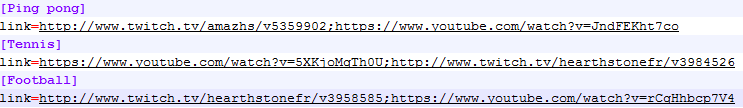
\includegraphics[width=1\textwidth]{inifile.png}
	\end{figure}
	
	
}

\section{Démonstration} 
\frame{\frametitle{Démonstration}
	\begin{figure}[h]
		\center
		
\includegraphics[width=0.6\textwidth]{play.png}
	\end{figure} 
	
}

\section{Conclusion \& perspectives}
\subsection{Conclusions}
\frame{\frametitle{Conclusions} 
	\begin{itemize}
		\item Application fonctionnelle
		\item Certaines fonctions non implémentée
	\end{itemize}

}
\subsection{Perspectives}
\frame{\frametitle{Perspectives} 
	\begin{itemize}
		\item Compléter les fonctions manquante
		\item Implémenter un bon nombre de sites
		\item Changer de langage
	\end{itemize}
	
}
	
\section{Questions} 
\frame{\frametitle{Questions} 
	\begin{figure}[h]
		\center
		
\includegraphics[width=0.4\textwidth]{Questions.png}
	\end{figure} 
}
\end{document}

